\documentclass[11pt,a4paper]{article}

\usepackage[utf8]{inputenc}
\usepackage[T1]{fontenc}
\usepackage[margin=2.5cm]{geometry}
\usepackage{hyperref}
\usepackage{xcolor}
\usepackage{listings}
\usepackage{tcolorbox}
\usepackage{booktabs}
\usepackage{fancyhdr}
\usepackage{enumitem}
\usepackage{tabularx}

% Definisi Warna
\definecolor{primary}{RGB}{18, 52, 86}
\definecolor{secondary}{RGB}{41, 128, 185}
\definecolor{darkgray}{RGB}{60, 60, 60}
\definecolor{lightgray}{RGB}{245, 247, 250}
\definecolor{bordercolor}{RGB}{210, 215, 220}
\definecolor{codebg}{RGB}{240, 243, 246}
\definecolor{accentgreen}{RGB}{39, 174, 96}
\definecolor{accentorange}{RGB}{230, 126, 34}

% Setup Hyperref
\hypersetup{
    colorlinks=true,
    linkcolor=secondary,
    filecolor=secondary,
    urlcolor=secondary,
    pdfauthor={UPT TIPD IAIN Parepare},
    pdftitle={Panduan Penggunaan dan Konfigurasi SIRITA SSO Sevima}
}

% Setup Header & Footer
\pagestyle{fancy}
\fancyhf{}
\fancyhead[L]{\small\textcolor{darkgray}{SIRITA SSO Sevima (Odoo 20) — Panduan Sistem}}
\fancyhead[R]{\small\textcolor{darkgray}{UPT TIPD IAIN Parepare}}
\fancyfoot[C]{\thepage}
\renewcommand{\headrulewidth}{0.4pt}

% Listing Style
\lstset{
    backgroundcolor=\color{codebg},
    basicstyle=\ttfamily\small,
    breaklines=true,
    frame=single,
    rulecolor=\color{bordercolor},
    keywordstyle=\color{secondary}\bfseries,
    stringstyle=\color{accentgreen},
    commentstyle=\color{darkgray}\itshape,
    showstringspaces=false
}

% Kotak Informasi & Peringatan
\newtcolorbox{infobox}[1][]{
    colback=lightgray,
    colframe=secondary,
    fonttitle=\bfseries,
    title=Informasi,
    #1
}

\newtcolorbox{warningbox}[1][]{
    colback=lightgray,
    colframe=accentorange,
    fonttitle=\bfseries,
    title=Peringatan Penting,
    #1
}

\newtcolorbox{successbox}[1][]{
    colback=lightgray,
    colframe=accentgreen,
    fonttitle=\bfseries,
    title=Keamanan \& Integritas Data,
    #1
}

\title{
    \vspace{-1.5cm}
    \textbf{\Huge \textcolor{primary}{PANDUAN LENGKAP PENGGUNAAN \& KONFIGURASI}}\\[0.3cm]
    \textbf{\Large Modul SIRITA SSO Sevima Platform (Odoo 20)}\\[0.2cm]
    \large Delegated Authentication \& Just-In-Time (JIT) Provisioning
}
\author{\textbf{UPT TIPD IAIN Parepare}}
\date{November 2026}

\begin{document}

\maketitle
\thispagestyle{fancy}

\begin{abstract}
Dokumen ini merupakan panduan teknis resmi implementasi dan operasional modul \textbf{SIRITA SSO Sevima} (\texttt{sirita\_sso\_sevima}) pada lingkungan ERP Odoo 20 IAIN Parepare. Modul ini memungkinkan seluruh sivitas akademika (Dosen, Tenaga Kependidikan, dan Mahasiswa) melakukan autentikasi ke Odoo menggunakan kredensial resmi Sevima SIAKAD Cloud, didukung oleh sinkronisasi otomatis \textit{Just-In-Time} (JIT) tanpa merusak atau menimpa integritas master data kepegawaian yang telah ada di modul HR.
\end{abstract}

\vspace{0.3cm}
\tableofcontents
\newpage

\section{Pendahuluan}

\subsection{Latar Belakang}
Dalam rangka mewujudkan ekosistem digital terpadu di lingkungan IAIN Parepare, sistem Enterprise Resource Planning (ERP) berbasis Odoo 20 diintegrasikan dengan sistem informasi akademik utama kampus (\textbf{Sevima Platform / SIAKAD Cloud}). Melalui modul \textbf{SIRITA SSO Sevima}, pengguna tidak lagi diwajibkan mengingat banyak username dan password, melainkan cukup menggunakan satu akun terpusat Sevima.

\subsection{Fitur Utama Modul}
\begin{enumerate}[label=\textbf{\arabic*.}]
    \item \textbf{Delegated Passthrough SSO}: Autentikasi real-time langsung ke API resmi Sevima Platform (\texttt{POST /siakadcloud/v1/user/login}).
    \item \textbf{Dual Login Identifier}: Pengguna dapat masuk menggunakan alamat \textbf{Email resmi} maupun \textbf{Nomor Induk Pegawai (NIP/NIDN)} atau \textbf{NIM}.
    \item \textbf{Just-In-Time (JIT) Auto-Provisioning}: Akun pengguna Odoo (\texttt{res.users}) otomatis dibuatkan saat pertama kali berhasil login jika opsi diaktifkan.
    \item \textbf{Smart HR Matching}: Menghubungkan akun login dengan profil pegawai (\texttt{hr.employee}) secara otomatis dan aman tanpa menimpa data yang telah ada.
    \item \textbf{Dual-Mode Fail-Safe}: Akun administrator lokal tetap dapat masuk menggunakan password internal Odoo apabila jaringan eksternal ke Sevima mengalami kendala.
    \item \textbf{Audit Trail \& Monitoring Log}: Seluruh riwayat percobaan login tercatat secara transparan dengan rincian waktu, alamat IP, latensi (ms), dan status respons.
\end{enumerate}

\subsection{Arsitektur \& Hubungan Antar Modul}
Modul \texttt{sirita\_sso\_sevima} dirancang mandiri (\textit{standalone}).
\begin{itemize}
    \item \textbf{Dependensi Inti}: Hanya bergantung pada modul standar Odoo: \texttt{base}, \texttt{web}, dan \texttt{hr}.
    \item \textbf{Interoperabilitas dengan \texttt{sirita\_sevima}}: Modul SSO tidak mewajibkan pemasangan modul \texttt{sirita\_sevima}. Namun jika \texttt{sirita\_sevima} telah terpasang, modul SSO memiliki mekanisme \textit{fallback} cerdas untuk meminjam konfigurasi API key secara otomatis jika kolom kredensial SSO belum diisi.
\end{itemize}

\newpage
\section{Konfigurasi Kredensial API di Backend}

Seluruh konfigurasi dapat diatur secara \textbf{dinamis} langsung melalui antarmuka web Odoo backend tanpa memerlukan perubahan berkas kode program maupun restart server.

\subsection{Kredensial API yang Diperlukan}
Untuk menghubungkan Odoo dengan Sevima Platform, Anda memerlukan data kredensial resmi dari Sevima:
\begin{table}[h!]
\centering
\small
\begin{tabularx}{\textwidth}{l p{4.5cm} X}
\toprule
\textbf{Parameter} & \textbf{Header HTTP / Kunci} & \textbf{Deskripsi} \\
\midrule
\textbf{Base URL} & — & URL endpoint API Sevima (\texttt{https://api.sevimaplatform.com}) \\
\textbf{App Key} & \texttt{X-App-Key} & Kunci identifikasi aplikasi resmi institusi dari Sevima \\
\textbf{Secret Key} & \texttt{X-Secret-Key} & Kunci rahasia otorisasi API \\
\bottomrule
\end{tabularx}
\caption{Kredensial API Sevima Platform}
\end{table}

\subsection{Langkah-Langkah Konfigurasi di Antarmuka Odoo}
\begin{enumerate}[label=\textbf{Langkah \arabic*:}]
    \item Masuk ke Odoo 20 menggunakan akun yang memiliki hak akses \textbf{Administrator}.
    \item Buka menu navigasi utama, lalu pilih \textbf{Settings} (\textit{Pengaturan}).
    \item Pada panel navigasi kiri, temukan dan klik sub-menu \textbf{SSO Sevima} (atau scroll ke bawah pada grup konfigurasi SIRITA SSO).
    \item Isi field konfigurasi sesuai data kredensial:
    \begin{itemize}
        \item \textbf{Aktifkan SSO Sevima Platform}: Centang (\textit{checklist}) untuk mengaktifkan mekanisme SSO.
        \item \textbf{Base URL API Sevima}: Masukkan \texttt{https://api.sevimaplatform.com} (atau URL sandbox/staging jika dalam tahap pengujian).
        \item \textbf{App Key}: Masukkan string App Key yang diberikan oleh Sevima.
        \item \textbf{Secret Key}: Masukkan string Secret Key yang sesuai.
        \item \textbf{Just-In-Time (JIT) Auto-Provisioning}: Centang opsi ini agar akun Odoo baru langsung dibuat saat pertama kali pegawai/mahasiswa login.
        \item \textbf{Batas Waktu Request (detik)}: Nilai default adalah \texttt{10} detik.
    \end{itemize}
    \item Klik tombol \textbf{Save} (\textit{Simpan}) di pojok kiri atas form Pengaturan.
\end{enumerate}

\subsection{Uji Koneksi Langsung (Live Connection Test)}
Sebelum mengumumkan ke seluruh pengguna, administrator dapat memvalidasi apakah kunci API dan koneksi jaringan berfungsi normal:
\begin{enumerate}
    \item Pada halaman pengaturan SSO Sevima yang sama, perhatikan bagian \textbf{Uji Koneksi \& Autentikasi Langsung}.
    \item Masukkan \textbf{Email Akun Uji Coba} dan \textbf{Password} akun Sevima yang aktif.
    \item Klik tombol \textbf{[Uji Login Akun Sevima]}.
    \item Sistem akan menampilkan notifikasi hasil uji:
    \begin{itemize}
        \item \textbf{Hijau (Sukses HTTP 200)}: Koneksi berhasil, kredensial valid, dan menampilkan nama pengguna serta peran akun uji coba beserta latensi koneksi (ms).
        \item \textbf{Kuning/Merah (HTTP 401 / 403)}: Kredensial akun uji coba salah atau App/Secret Key ditolak oleh API Sevima.
    \end{itemize}
\end{enumerate}

\newpage
\section{Perilaku Sistem terhadap Master Data Pegawai (HR)}

\begin{successbox}
\textbf{Prinsip Integritas Master Data:}
Modul \texttt{sirita\_sso\_sevima} \textbf{TIDAK AKAN} menimpa (\textit{overwrite}) maupun menghapus data pegawai yang telah ada di tabel \texttt{hr.employee}.
\end{successbox}

\subsection{Alur Pencocokan Pegawai (\textit{Employee Matching})}
Ketika seorang pegawai (Dosen atau Tenaga Kependidikan) login menggunakan kredensial Sevima, sistem menjalankan alur sebagai berikut:

\begin{enumerate}
    \item \textbf{Ekstraksi Data Respons API}: Mengambil atribut NIP, ID Pegawai, Nama, Email, dan Role dari respons Sevima.
    \item \textbf{Pencarian Data di \texttt{hr.employee}}:
    \begin{itemize}
        \item Sistem mencari pegawai di tabel \texttt{hr.employee} yang memiliki kesesuaian nilai NIP pada kolom \texttt{barcode} atau \texttt{identification\_id}.
        \item Jika NIP tidak ditemukan, sistem mencoba mencocokkan berdasarkan kolom \texttt{work\_email}.
    \end{itemize}
    \item \textbf{Penautan Otomatis (\textit{Safe Linking})}:
    \begin{itemize}
        \item Jika record pegawai ditemukan dan field \textbf{Related User} (\texttt{user\_id}) masih kosong, sistem akan mengisinya dengan ID user Odoo yang baru dibuat.
        \item Jika field \texttt{user\_id} pada pegawai tersebut sudah ada, sistem \textbf{tidak akan mengubahnya}.
        \item Kolom master lainnya (Nama, Jabatan, Departemen, Tempat/Tanggal Lahir, SK, dll.) \textbf{tetap utuh 100\%}.
    \end{itemize}
    \item \textbf{Penambahan Atribut Metadata SSO}:
    Sistem hanya melengkapi informasi metadata pendukung:
    \begin{itemize}
        \item \texttt{sevima\_user\_id}: ID unik akun pengguna di Sevima.
        \item \texttt{is\_sevima\_synced}: Ditandai bernilai \texttt{True}.
    \end{itemize}
\end{enumerate}

\subsection{Penentuan Hak Akses Pengguna Baru (Role Mapping)}
Secara cerdas, modul ini membedakan jenis pengguna berdasarkan kode peran dari Sevima:
\begin{itemize}
    \item \textbf{Dosen (\texttt{DSN}) \& Tendik (\texttt{TDK} / \texttt{PEG})}:
    Otomatis diberikan hak akses \textbf{Internal User} (\texttt{base.group\_user}) sehingga dapat mengakses modul-modul internal Odoo seperti Kepegawaian, Cuti, dan Presensi.
    \item \textbf{Mahasiswa (\texttt{MHS})}:
    Otomatis dialokasikan ke kelompok \textbf{Portal User} (\texttt{base.group\_portal}) sehingga hanya dapat mengakses halaman portal terbatas.
\end{itemize}

\newpage
\section{Panduan Pengoperasian Bagi Pengguna Akhir}

\subsection{Tampilan Antarmuka Halaman Login}
Halaman login portal ERP IAIN Parepare telah terintegrasi secara dinamis dengan identitas lembaga dan SSO. Di bagian atas formulir login, pengguna disuguhkan banner notifikasi resmi \textbf{"Login menggunakan SSO Sisfokampus atau Edlink"}.

\begin{figure}[h!]
\centering
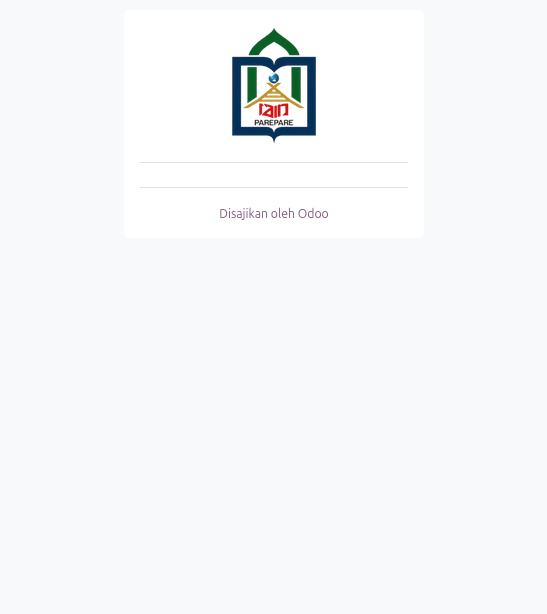
\includegraphics[width=0.62\textwidth]{image.png}
\caption{Antarmuka Halaman Login Portal IAIN Parepare (portal.iainpare.ac.id)}
\label{fig:login_portal}
\end{figure}

\subsection{Cara Masuk Menggunakan Akun Sisfokampus / Edlink (Email)}
\begin{enumerate}
    \item Buka URL portal resmi di \textbf{\url{https://portal.iainpare.ac.id/web/login}}.
    \item Masukkan \textbf{Email Resmi} yang terdaftar di akun Sisfokampus / Sevima / Edlink pada kolom \textit{Email}.
    \item Masukkan \textbf{Password Akun} Anda pada kolom \textit{Password}.
    \item Klik tombol \textbf{Log in}. Sistem akan memvalidasi langsung ke server Sevima secara aman dan otomatis mengarahkan ke dashboard.
\end{enumerate}

\subsection{Cara Masuk Menggunakan NIP / NIDN}
\begin{enumerate}
    \item Pada halaman login Odoo, masukkan \textbf{NIP atau NIDN} langsung pada kolom \textit{Email}.
    \item Masukkan kata sandi akun Sisfokampus / Edlink Anda.
    \item Modul secara otomatis meresolusi NIP tersebut ke akun email kerja yang terdaftar di master data kepegawaian kampus sebelum memverifikasi kredensial.
    \item Setelah validasi berhasil, akun sesi login akan aktif secara otomatis.
\end{enumerate}

\subsection{Mekanisme Fail-Safe Administrator Lokal}
\begin{warningbox}
Jika server API Sevima sedang dalam masa pemeliharaan (\textit{maintenance}) atau terjadi gangguan jaringan internet internasional:
\begin{itemize}
    \item Akun Administrator internal Odoo (misal: \texttt{admin}) \textbf{tetap dapat login} menggunakan password lokal database Odoo.
    \item Sistem otomatis beralih ke pengecekan password lokal jika autentikasi SSO mengalami kegagalan atau timeout.
\end{itemize}
\end{warningbox}

\newpage
\section{Audit Trail \& Monitoring Log Autentikasi}

Seluruh aktivitas login melalui SSO Sevima dicatat secara komprehensif untuk keperluan audit keamanan TI dan evaluasi kinerja jaringan.

\subsection{Melihat Log Login SSO}
\begin{enumerate}
    \item Masuk ke menu \textbf{Settings} $\rightarrow$ \textbf{Technical} $\rightarrow$ \textbf{Audit Log SSO Sevima}.
    \item Atau akses cepat melalui menu Pengaturan SSO dengan mengklik tombol \textbf{Lihat Audit Log SSO}.
    \item Daftar rekaman log menyajikan rincian:
    \begin{itemize}
        \item \textbf{Tanggal \& Waktu}: Waktu presisi percobaan login.
        \item \textbf{Input Login}: Email atau NIP yang dimasukkan.
        \item \textbf{Status}: \texttt{SUCCESS} (hijau) atau \texttt{FAILED} (merah).
        \item \textbf{Latency (ms)}: Waktu respons server API Sevima dalam milidetik.
        \item \textbf{IP Address}: Alamat IP asal pengguna.
        \item \textbf{Peran \& Satker}: Role akun yang berhasil terautentikasi.
        \item \textbf{Raw Response}: Cuplikan respons mentah dari server API untuk investigasi teknis.
    \end{itemize}
\end{enumerate}

\section{Pemecahan Masalah (Troubleshooting)}

\begin{table}[h!]
\centering
\small
\begin{tabularx}{\textwidth}{l p{4cm} X}
\toprule
\textbf{Gejala / Kode} & \textbf{Kemungkinan Penyebab} & \textbf{Langkah Penyelesaian} \\
\midrule
\textbf{HTTP 401} & Password salah atau akun belum aktif di Sevima. & Pastikan pengguna dapat login di portal web SIAKAD Cloud. Periksa atribut \texttt{status\_aktif} akun. \\
\addlinespace
\textbf{HTTP 403} & App Key atau Secret Key tidak valid. & Periksa kembali konfigurasi App Key dan Secret Key di menu Settings Odoo. \\
\addlinespace
\textbf{Timeout (>10s)} & Gangguan koneksi internet server atau firewall kampus. & Periksa koneksi outbound server Odoo ke \texttt{api.sevimaplatform.com}. Tambah batas timeout jika koneksi lambat. \\
\addlinespace
\textbf{User Odoo Tidak Terbentuk} & Fitur JIT Auto-Provisioning belum diaktifkan. & Buka menu Settings $\rightarrow$ SSO Sevima, centang opsi \textit{Just-In-Time (JIT) Auto-Provisioning User}, lalu simpan. \\
\addlinespace
\textbf{Pegawai Tidak Terhubung} & NIP atau Email di Sevima berbeda dengan di \texttt{hr.employee}. & Pastikan kolom \texttt{barcode} atau \texttt{identification\_id} pada master pegawai diisi dengan NIP yang sama persis. \\
\bottomrule
\end{tabularx}
\caption{Tabel Panduan Pemecahan Masalah}
\end{table}

\vspace{1cm}
\begin{center}
\small
\textcolor{darkgray}{Dokumen Resmi Sistem Informasi SIRITA — UPT TIPD IAIN Parepare}\\
\textit{Dipublikasikan untuk standarisasi operasional ERP Odoo 20.}
\end{center}

\end{document}
